\documentclass[crop]{standalone}

\usepackage{amsmath}

\usepackage{tikz}

\usetikzlibrary{shapes,decorations,arrows,calc,arrows.meta,fit,positioning}
\tikzset{
    -Latex,auto,node distance =1 cm and 1 cm,semithick,
    O/.style ={rectangle, draw, minimum width = 0.7 cm},
    U/.style ={rectangle, draw, minimum width = 0.7 cm, dashed},
    point/.style = {circle, draw, inner sep=0.04cm,fill,node contents={}},
    bidirected/.style={Latex-Latex,dashed},
    el/.style = {inner sep=2pt, align=left, sloped}
}

\begin{document}


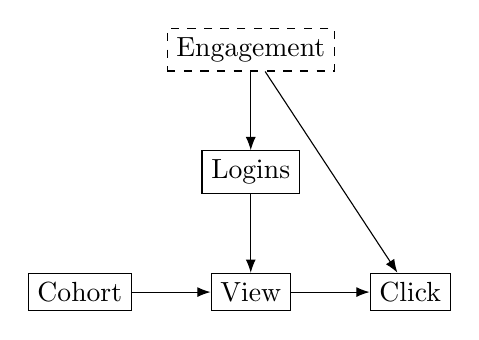
\begin{tikzpicture}
  \node[O] (x) at (0,0) {Cohort};
  \node[O] (m) [right =of x] {View};
  \node[O] (y) [right =of m] {Click};
  \node[O] (l) [above =of m] {Logins};
  \node[U] (c) [above =of l] {Engagement};
  \path (x) edge (m);
  \path (m) edge (y);
  \path (c) edge (y);
  \path (c) edge (l);
  \path (l) edge (m);

\end{tikzpicture}

\end{document}
